%
% Copyright (C) 2020 Jan Nowotsch
% Author Jan Nowotsch	<jan.nowotsch@gmail.com>
%
% Released under the terms of the GNU GPL v2.0
%



\section{Integration Test Framework}
	The integration test framework is intended to test kernel and user space in combination. Figure~\ref{fig:int_test_framework} summarises the main components of the framework.

	\begin{figure}[h]
		\centering	
		\includegraphics[scale=.75]{test/int_test_framework}
		\caption{Integration test framework components.}
		\label{fig:int_test_framework}
	\end{figure}

	The framework uses one process each for the kernel, the user space application and the actual framework itself. The interface between those processes are \gls{ipc} pipelines and signals which emulate hardware events/operations, such as interrupts and hardware state controls.

	The integration test framework process implements threads with the following responsibilities:
	\begin{description}
		\item[Signal Handler] Processing of hardware requests from the kernel and user space processes. Application state handling, especially shutdown and broken communication to the kernel and user space processes.

		\item[Hardware Event Handler] Process hardware events.
		\item[Interrupt Controller] Trigger hardware requests to the kernel.
		\item[Timer] Periodically enqueue timer interrupts.
		\item[User Input] In interactive mode the framework is controlled by user inputs, which are handled by this thread.
	\end{description}

	The kernel and user space processes are single-threaded. Hence, the only mechanism to interact with them is through signal handlers. Signal handlers cannot be interrupted themselves, thus the protocol used for hardware operations and the mutex between the hardware event handler and the interrupt controller thread ensure that there is only a single ongoing hardware event.

	\subsection{Hardware Event/Operation Protocol}
		Figure~\ref{fig:int_test_protocol} depicts the protocol to trigger, process and complete a hardware operation.

		\begin{figure}[h]
			\centering	
			\includegraphics[scale=.75]{test/int_test_protocol}
			\caption{Hardware event/operation protocol.}
			\label{fig:int_test_protocol}
		\end{figure}

		An operation is initiated by the requester sending one of the \gls{ipc} signals to the target. For synchronisation and to acknowledge the request the target sends a sequence number. The requester blocks until the sequence number is available. Once synchronised the actual operation data are exchanged.

		During processing further data might be exchanged.

		Once processing is complete the operation's write-back phase is again used for synchronisation. The requester blocks while waiting for the results being transfered. The target writes the results. To acknowledge the reception of the results, the requester responds with a sequence number which is read by target.

		Upon completion of the write-back phase both, requester and target, are known to have completed all relevant operations and are clear to trigger or accept a new operations.
